%%% Commandes perso

\newcommand{\trou}[1]{\gap*{#1}}% pour texte à trou avec pointillés
\newcommand{\troub}[1]{\gap*[b]{#1}}% pour texte à trou avec blanc
\newcommand{\troum}[1]{\text{\gap*{$#1$}}}% pour texte à trou avec pointillés dans envirronnement math
\newcommand{\troubm}[1]{\text{\gap*[b]{$#1$}}}% pour texte à trou avec blanc dans envirronement math
\DeclareMathAlphabet{\mathbbb}{U}{fplmbb}{m}{n} %% symboles ensembles maths normaux

% lignes de pointillés à compléter
\newcommand{\dotsfill}[1]{
    \foreach \n in {1,...,#1} {
        .\dotfill \\
    }
}

% fonction
\newcommand{\fonction}[5]{
	\begin{array}[t]{l|rcl}
		#1: & #2 & \longrightarrow & #3 \\
			& #4 & \longmapsto 	& #5
	\end{array}
}

\newcommand{\calculatrice}{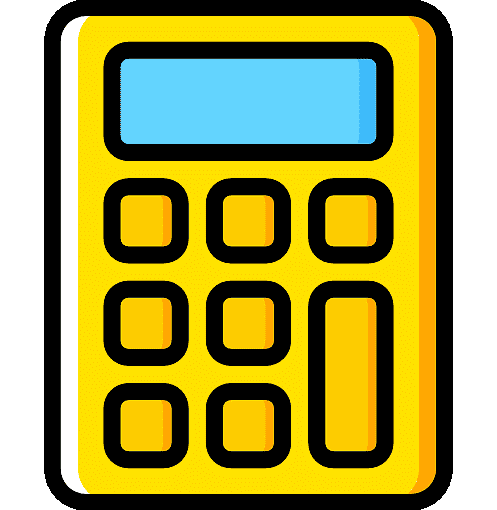
\includegraphics[width=13pt]{icons/calc.png}}
\newcommand{\nocalculatrice}{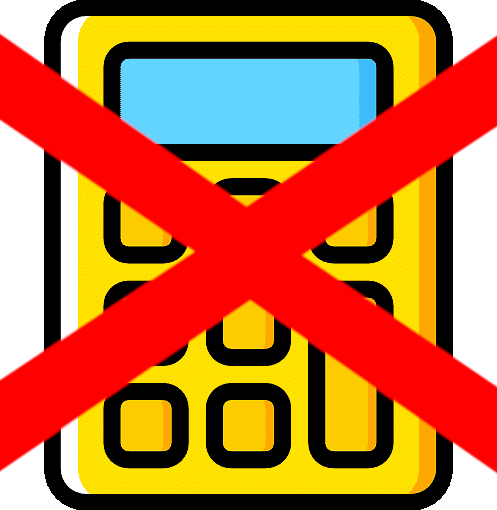
\includegraphics[width=13pt]{icons/nocalc.png}}
\newcommand{\I}{\noindent}
\newcommand{\euro}{\eurologo{} }
\DeclareMathOperator{\ent}{E}
\DeclareMathOperator{\ch}{ch}
\DeclareMathOperator{\sh}{sh}
\newcommand{\R}{\mathbbb{R}}
\newcommand{\N}{\mathbbb{N}}
\newcommand{\D}{\mathbbb{D}}
\newcommand{\Z}{\mathbbb{Z}}
\newcommand{\Q}{\mathbbb{Q}}
\newcommand{\Cx}{\mathbb{C}} % nombres complexes 
\newcommand{\U}{\mathbb{U}} % nombres complexes 
\newcommand{\C}{\mathcal{C}} % attention ce ne sont pas les complexes!!
\newcommand{\M}[2]{\mathcal{M}_{#1,#2}} % ensemble de matrices
\newcommand{\Mnp}{\mathcal{M}_{n,p}} % ensemble de matrices de taille n x p
\newcommand{\Mn}{\mathcal{M}_{n}} % ensemble de matrices carrée de taille n
\newcommand{\tr}[1]{{}^t#1} % transposée d'une matrice
\newcommand{\E}{\text{E}} % partie entière
\renewcommand{\Re}{\text{Re}} % partie réelle
\renewcommand{\Im}{\text{Im}} % partie imaginaire
\renewcommand{\arg}{\text{arg}} % argument
\newcommand{\mdpi}{~[2\pi]} % modulo 2\pi
\newcommand{\mpi}{~[\pi]} % modulo 2\pi
\renewcommand{\P}{\mathcal{P}} 
\newcommand{\Qcal}{\mathcal{Q}} 
\renewcommand{\S}{\mathcal{S}} 
\newcommand{\B}{\mathcal{B}} 
\renewcommand{\bf}[1]{\textbf{#1}}
\newcommand{\gs}{\geqslant}
\newcommand{\ls}{\leqslant}
% \newtcbox{\hl}{on line,
% 	arc=4pt,colback=myorange!40!white,colframe=myorange,
% 	before upper={\rule[-3pt]{0pt}{10pt}},boxrule=1pt,
% 	boxsep=0pt,left=6pt,right=6pt,top=2pt,bottom=2pt}
%\newcommand{\hl}[1]{\colorbox{myorange!40!white}{#1}}
\newcommand{\hlp}[1]{\colorbox{mypurple!40!white}{#1}}
\newcommand{\hlg}[1]{\colorbox{gray!40!white}{#1}}

\renewcommand{\r}[1]{\textcolor{myred}{#1}}
\renewcommand{\b}[1]{\textcolor{myblue}{#1}}
\newcommand{\g}[1]{\textcolor{mygreen}{#1}}
\newcommand{\p}[1]{\textcolor{mypurple}{#1}}
\newcommand{\limn}{\lim\limits_{n\to+\infty}}
\newcommand{\V}[1]{\ensuremath{\overrightarrow{\,\mathstrut#1\,}}}
\renewcommand{\v}[1]{\ensuremath{\vec{#1}} }
\newcommand{\para}{/\!/}
\newcommand{\vect}[2]{\left(\begin{array}{c}#1\\#2\end{array}\right)}
\newcommand{\veci}{\v{i}}
\newcommand{\vecj}{\v{j}}
\newcommand{\veck}{\v{k}}
\newcommand{\vecu}{\v{u}}
\newcommand{\vecv}{\v{v}}
\newcommand{\vecw}{\v{w}}
\newcommand{\vecn}{\v{n}}
\newcommand{\norm}[1]{||#1||}
\newcommand{\bijk}{\veci,\vecj,\veck}
\newcommand{\oij}{(O\,;\,\veci\,,\,\vecj)}
\newcommand{\oijk}{(O\,;\,\veci\,,\,\vecj\,,\,\veck)}
\newcommand{\ouv}{(O\,;\,\vecu\,,\,\vecv)}
\newcommand{\coordvp}[2]{\begin{pmatrix}#1\\#2\end{pmatrix}} %vecteur du plan
\newcommand{\coordv}[3]{\begin{pmatrix}#1\\#2\\#3 \end{pmatrix}} % vecteur de l'espace
\newcommand{\coordpp}[2]{\left(#1\,;\,#2\right)} % point du plan
\newcommand{\coordp}[3]{\left(#1\,;\,#2\,;\,#3\right)} % point de l'espace
\newcommand{\limp}{\lim\limits_{x\to+\infty}} % limite en + infinie
\newcommand{\limm}{\lim\limits_{x\to-\infty}} % limite en - infinie
\newcommand{\lima}[1]{\lim\limits_{x\to #1}} % limite en a
\newcommand{\limcomp}[2]{\lim\limits_{#1\to #2}} % limite pour composée
\newcommand{\limd}[1]{\lim\limits_{\substack{x \to#1 \\ x>#1}}} % limite en a à droite
\newcommand{\limg}[1]{\lim\limits_{\substack{x \to#1 \\ x<#1}}} % limite en a à gauche
\renewcommand{\angle}[1]{\widehat{#1}}
\newcommand{\card}{\text{Card}}
\newcommand{\flocon}{\ding{100}}
\newcommand{\cm}{\text{ cm}}
\newcommand{\dm}{\text{ dm}}
\newcommand{\km}{\text{ km}}
\newcommand{\m}{\text{ m}}
\newcommand{\droiteparam}[4][, t\in\R]{\left\{\begin{array}{ll}#2&\\#3&#1\\#4&\end{array}\right.}
\renewcommand{\det}[2]{\text{det}(#1\,,\,#2)}
\newcommand{\detm}{\text{det}} % determinant matrice
\newcommand{\Det}[1]{\begin{vmatrix}#1\end{vmatrix}}
\newcommand{\fleche}{\ding{220}}
\renewcommand{\bar}[1]{\overline{#1}}
\newcommand{\chevron}{{>}{>}{>} }
\newcommand{\bfrac}[2]{\dfrac{#1}{~#2~}} % grande barre de fraction
\newcommand{\e}{\text{e}} % constante d'Euler
\newcommand{\pgcd}[2]{\text{PGCD}(#1\,;\,#2)} % PGCD
\newcommand{\ensDcom}[2]{\text{D}(#1\,;\,#2)} % ensemble des diviseurs communs
\newcommand{\ensD}[1]{\text{D}(#1)} % ensemble des diviseurs
\newcommand{\ppcm}[2]{\text{PPCM}(#1\,;\,#2)} % PPCM
\newcommand{\bz}{\bar{z}} % conjugué de z
\newcommand{\rz}{\Re(z)} % partie réelle de z
\newcommand{\iz}{\Im(z)} % partie imaginaire de z
\newcommand{\trig}[2]{#1\left(\cos\left(#2\right)+i\sin\left(#2\right)\right)} % forme trigonometrique
\newcommand{\mat}[1]{\begin{pmatrix}
		#1
\end{pmatrix}} % matrice
\newcommand{\syst}[1]{
	\left\{\begin{array}{rcl}
		#1
\end{array}\right.
} % systeme lineaire

\newcommand{\systl}[1]{
	\left\{
	\begin{array}{rcll}
		#1
	\end{array}
	\right.
} % systeme lineaire avec lignes

\newcommand{\dpar}[2]{\dfrac{\partial #1}{\partial #2}}

%% Symboles
\newcommand{\pen}{\ding{46}~}
\newcommand{\ok}{\textcolor{mygreen}{\ding{51}}~}
\newcommand{\notok}{\textcolor{myred}{\ding{55}}~}
\newcommand{\attention}{\textdbend}
\newcommand{\demonstration}{
\includegraphics[width=12pt]{icons/demo.png}}

% Intervalles
% ***********
\newcommand{\intervalle}[4]{\mathopen{#1}#2\mathclose{}\mathpunct{};#3\mathclose{#4}}
\newcommand{\ff}[2]{\intervalle{[}{#1}{#2}{]}}
\newcommand{\of}[2]{\intervalle{]}{#1}{#2}{]}}
\newcommand{\fo}[2]{\intervalle{[}{#1}{#2}{[}}
\newcommand{\oo}[2]{\intervalle{]}{#1}{#2}{[}}
\newcommand{\bff}[2]{\intervalle{\biggl[}{#1}{#2}{\biggr]}}
\newcommand{\bof}[2]{\intervalle{\biggl]}{#1}{#2}{\biggr]}}
\newcommand{\bfo}[2]{\intervalle{\biggl[}{#1}{#2}{\biggr[}}
\newcommand{\boo}[2]{\intervalle{\biggl]}{#1}{#2}{\biggr[}}

% Intervalles entiers
% ***********
\newcommand{\ffi}[2]{\intervalle{[\![}{#1}{#2}{]\!]}}
\newcommand{\ofi}[2]{\intervalle{[\![}{#1}{#2}{]\!]}}
\newcommand{\foi}[2]{\intervalle{[\![}{#1}{#2}{]\!]}}
\newcommand{\ooi}[2]{\intervalle{[\![}{#1}{#2}{]\!]}}
